\begin{frame}[t]
  \frametitle{HanKa -- V \& V}
  \vspace*{-.3cm}
  \centering\textcolor{structure.bg!95!blue}{ Assembly average power distribution comparisons }\\[-.3em]
  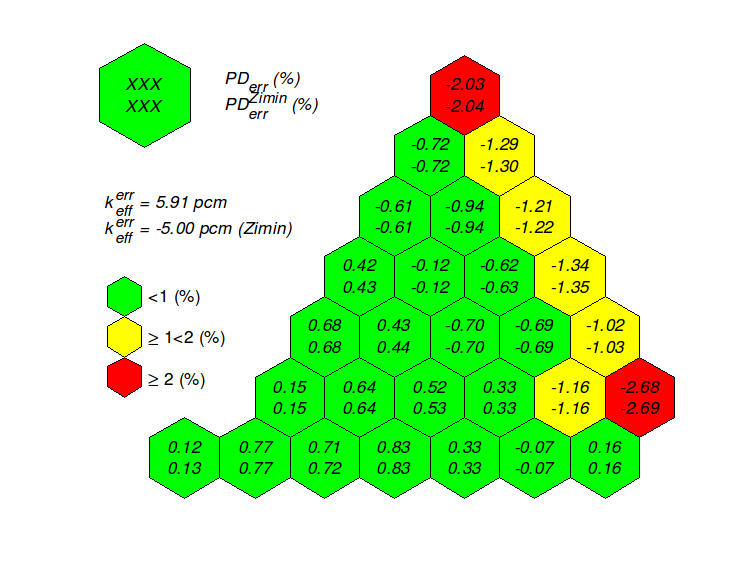
\includegraphics[scale=.5]{images/HanKa/HCZ1T.png}
  \vspace{-.7cm} \hrule width 5.1cm \vspace{-0.1cm}
	\begin{thebibliography}{\textwidth} 
	  \beamertemplatearticlebibitems
		\bibitem{ZiminBaturin02}
    {\scriptsize V.~G.~Zimin and D.~M.~Baturin}
    \newblock {\scriptsize Polynom. Nod. Meth. for Solving Neutron Dif. Eqns. in Hex-Z Geometry}. 
    \newblock {\scriptsize \color{white!80!black}Ann. Nucl. En. 29 (2002)}
	\end{thebibliography}
\end{frame}

\begin{frame}[t]
  \frametitle{HanKa -- V \& V}
  \vspace*{-.3cm}
  \centering\textcolor{structure.bg!95!blue}{ Assembly average power distribution comparisons}\\[-.3em]
  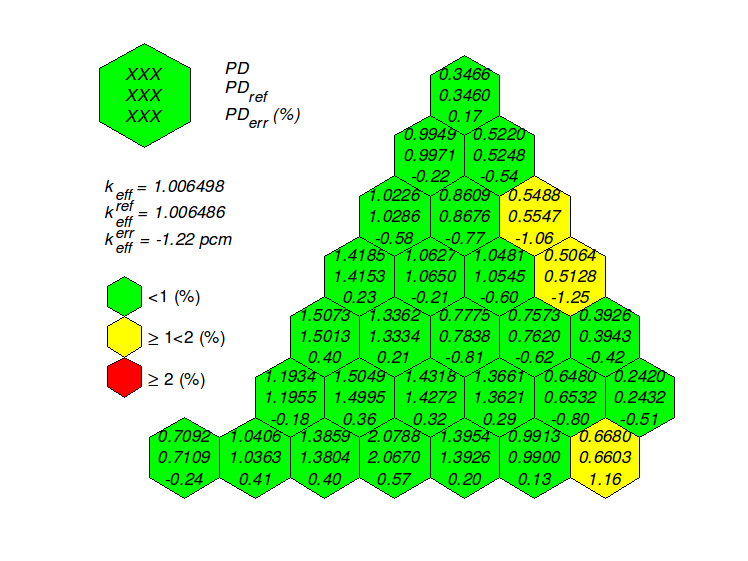
\includegraphics[scale=.5]{images/HanKa/HCZ2T.png}
  \vspace{-.85cm} 
  \begin{center} Modified treatment of boundary nodes \end{center}
\end{frame}
